\documentclass[a4paper, openany]{memoir}

\usepackage[utf8]{inputenc}
\usepackage[T1]{fontenc} 
\usepackage[english]{babel}
\usepackage{amsmath}
\usepackage{amssymb}

\usepackage{booktabs}
\usepackage{fancyhdr}
\usepackage{float}
\usepackage{indentfirst}
\usepackage{graphicx}
\usepackage[linewidth=1pt]{mdframed}
\usepackage{multicol}
\usepackage{fancyvrb}

\usepackage{longtable}

\pagestyle{fancy}
\fancyhf{}
\fancyhead[LE]{\leftmark}
\fancyhead[RO]{\rightmark}
\fancyhead[RE, LO]{PSD}
\fancyfoot[LE, RO]{\thepage}
\fancyfoot[RE, LO]{Pete Gautam}

\renewcommand{\headrulewidth}{1.5pt}

\setcounter{chapter}{16}
\chapterstyle{thatcher}

\begin{document}
\chapter{Software licensing}
A licence is an assertion of the permitted uses of a software artifact and its conditions of use. A licence may cover a range of topics, such as:
\begin{itemize}
    \item ownership of the software artifact
    \item end usage rights such as display and performance
    \item distribution rights, such as reproductive, which is usually covered by copyright
    \item engineering rights, such as disassembly, modification and incorporation in other software
    \item warranties and liability.
\end{itemize}

At the most abstract level, there are 2 roles in licensing: the provider and the consumer of the artifact. Producers of the software may be the original authors, but there are lots of other ways people can be involved in production. For example, the owner of a copy of an artifact is distinct from the original author. It may be important to establish in the licence who has ownership of a software copy. Similarly, a licence might be applied by a distributor of a software artifact who was not the original author. A repository hosting site might impose condition on hosting, for example. 

On the other side of the relationship, there may be several types of consumers, and a licence may address them differently. A licence might refer to what a customer (who is acquiring the software in some way) may have rights to. For example, the licence may state whether the customer is acquiring ownership of a copy of the software, or if they are just acquiring the right to use it for some purpose, or even just for a limited period of time. 

Infrastructure engineers may be consumers of licences because they are responsible for installing and configuring software on behalf of end users. They may need to ensure that the configured environment complies with licences during this process, and that there are no conflicts between licences. End users are part of the licence because it often describes the permitted and non-permitted usage of the software. For example, some software producers offer academic licences, allowing the software to be used at reduced or no cost, provided that it is only used in an educational setting or purpose. Developers may also be consumers of software licence if they incorporate a software produced by others in their work.

\section{Licence ecosystem}
Since software exists in an ecosystem, most participants undertake roles as both producers and consumers of software and their respective licences, as shown below.
\begin{figure}[H]
    \centering
    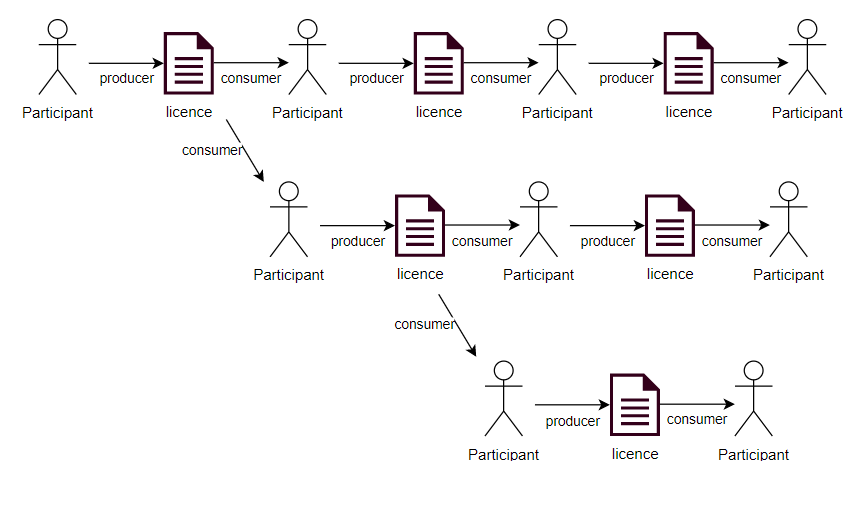
\includegraphics[scale=0.6]{src/17.1 licence ecosystem.PNG}
\end{figure}
\noindent We can think of licensing in a network of consumer-producer relationships. Any given producer of a licence may also be a consumer of a licence, as provided by others if they incorporate their software into their own work. This is why software licensing is so important. Even if we do not explicitly apply a licence to a software, we may still be affected by licences applied to other softwares that the project depends on.

In addition, even if we do not apply a licence to a software, it does not automatically mean that it will treated as being in the public domain. In some jurisdictions, restrictions on use and contribution of created work is automatic. So, by not applying a licence, we may be more restrictive than we mean to.

A further complication is that licensing structures may contain cycles. A simple example is JUnit. JUnit depends on the assertion framework Hamcrest, and Hamcrest uses JUnit for test. So, the JUnit team must satisfy the Hamcrest licence condition, and vice versa. In this case, there is no difficulty as the two licences are compatible.

A licence can be applied to almost any software artifact. A licence may refer to any of the associated artifacts on a software project, such as the source code, binaries, documentation and outputs. However, not everything covered in a licence will be applicable to all the kinds of artifacts.

\section{Copyright}
Copyright is a form of intellectual property (IP). Other examples of IP are trademark and pattern. Copyright is the legal right to control reproduction of created work for a limited period of time. The length of time depends on the jurisdiction, but is typically at least 50 years after publication or the author's death.

A key concept in copyright is derivation. This is because, in many jurisdictions, a copyright holder is also entitled to copyright on any derivative works. For the purposes of software, derivative is commonly thought to mean modifications to the existing source code base. The Copyright, Designs and Patents Act (1988) codifies derivation.

Without specific authorisation in a licence, it is generally not permitted to attempt to make modifications to a copyrighted work. In software terms, this is generally taken to mean actions like decompiling code and making modifications to the resulting source code. 

It is important to emphasise that copyright does not prevent copying, distribution and modification of a software artifact. It just means that the original author has the right to decide under what conditions this may be done and document them in a licence to consumers.

\begin{figure}[H]
    \centering
    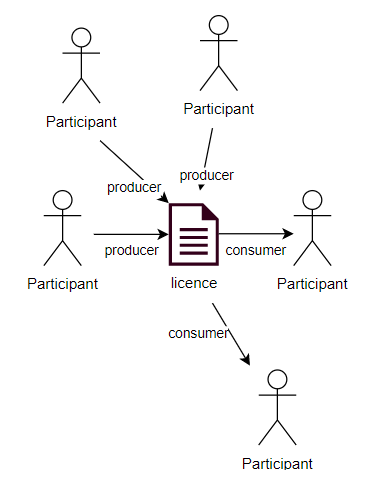
\includegraphics[scale=0.7]{src/17.2 contributors copyright.PNG}
\end{figure}
\noindent The diagram above shows how several different producers may make contributions to a single software artifact. In this case, the copyright for the contributions may be held, in the first instance, by the contributor. To handle for this, contributors can be asked to assign their copyright to the project's owner. This may be through the contract of employment. 

In the case of an open source project, the licence of the original software may require derivations (i.e. contributions) to be licensed under the same terms. In this case, the licence may require copyright to be transferred to the original project author or the copyright becomes shared between all the contributors.

In both cases, the interest of the contributor is protected by ensuring that when they make a contribution, they will continue to be able to access and re-distribute the software system. One downside of having multiple copyright holders is that it may make protection of the copyright harder to defend.

Open source contribution is a particular example of the effective derivation, but there are others:
\begin{itemize}
    \item If an existing work of source code $P$ is incorporated into another source codebase $C$, then this may count as derivation. Factors to consider are the extent to which the functionality of $C$ is dependent on the functionality of $P$. A single line of code producing a logging statement might not be considered derivation, for example. Alternatively, if an existing library is incorporated into the project through some form of linking mechanism, then this may also be considered derivation. Again, this may depend on how dependent the linking program is on the library.
    
    \item Some types of programs may themselves be used to produce programs or different representations of programs. Sometimes, these programs may incorporate portions of their own implementation in the generated program. Obvious examples are compilers and parser generators. In these cases, the generated program and its representation may be considered a derived work. We do not typically considered outputs as derived works. Using an IDE to develop a new software would also not by itself make the software application a derived work of the IDE. This is only the case if it contains substantial material that originated in the IDE program.
\end{itemize}

\subsection{Copyleft}
Given this very general nature of derivation, the terms of software licence can also be transitive. This means that if a software artifact is incorporated into another software project, some or all of its licence conditions may also need to be imposed on the consumers of the incorporating software. This is something referred to as viral licensing- the licence terms may come to affect software some distance away in the ecosystem.

\section{Warranty and Liability}
Warranties and liabilities are also covered in software licences. A warranty asserts that the period of time in which the consumer can expect a product to function without exhibits defects. Many FOSS (Free and Open Source Software) licences, and even proprietary and commercial licences assert that a software has no warranty. So, the cost of fixing any defects lies with the customer.

In practice, many licences commit providers to supplying updates for a fixed period of time. That way, they can fix defects that become apparent during that period. Licences may also warrant that the software performs as described in the associated literature. So, the customers are allowed to seek redress if this is not the case.

Liability clauses are opposite of warranties. They state who is responsible if the software has defects and causes damages. FOSS licences often assert that the customer is responsible for any damages.

\section{Enforcement}
A software licence is an assertion of the expectations as to the use of the software. It isn't an absolute rule. If we impose restrictions on the distribution, usage and modification of software, it does not necessarily mean that they will be automatically obeyed. Licencers often have to take additional steps to enforce licence conditions.

These can be broadly categorised as implementing technical measures to prevent a violation or monitoring for violations and seeking redress through a legal process. The first approach for a producer is to implement technical mechanisms that are able to prevent a licence condition being breached. The nature of the measures taken depends on the condition we are trying to guarantee. For example, reproduction conditions may be enforced through the use of a rights management software. Making programs harder to modify by using just in time decryption and preventing unauthorised usage through licence servers and subscription mechanisms is also possible.

If seeking to enforce a licence through legal arbitration process, the first issue is that we need to know a violation has occurred. Technical measures may help here, depending on the licence condition we are seeking to enforce. For example, we can detect unauthorised distribution using file shared systems,  monitoring and finger printing technology.

\subsection{Reputational issues}
Licence conditions and enforcement mechanisms that are unreasonable may cause reputational damage for the software. For example, software licences may require users to provide access to extensive personal information stored in the same device, or access to accounts for services. This information is often valuable as part of the business model for the provider, but may cause reputational harm if widely reported.

It may be tempting to deny updates to end users who violate the licence conditions, e.g. by not paying for a subscription. However, this is risky. The software used to determine whether the licence has been procured or not may be defective. Also, if the update addresses as software vulnerability, it means that not all the running instances of the software are patched. This leads the user base (as a whole) more vulnerable to attack.

It may also be tempting to install monitoring software on an end user's device that actively prevents them from violating the terms of the licence, by modifying and disabling some other softwares. This is likely to annoy legitimate users who may have good reasons for the functionality. In addition, it may expose their devices to vulnerabilities created by the monitoring software.

Legal redress may well be effective if the parties in both cases are large organisations with significant resources. This is required to cover both the legal costs and any fines incurred. However, if one party is substantially larger than another, this may cause reputational issues for the larger organisation, especially if it is attempting to seek redress from the smaller, more vulnerable entity.

\section{Considerations for licence}
Licences are a means of maximising benefit to the distributor of software by controlling what usage others can make of it. However, the more restrictions that are placed on the use of a software project, the less attractive the proposition becomes for the consumer. In addition, the more the restrictions, the more likely it is that violations will occur. Thus, we require more investment for enforcing on behalf of the provider.

Therefore, selection of a licence is a trade-off between:
\begin{itemize}
    \item the desire to make a product attractive to consumers, by being permissive in ways that might risk the viability of the business model, and
    \item the ability of the distributor to enforce any conditions applied.
\end{itemize}

So, a number of questions can be asked when trying to choose a licence:
\begin{itemize}
    \item Who are the target end users of the software?
    \item Do we want the software to be used within other projects? If so, how can we incentivise it?
    \item Who are the customers? What are their resources?
    \item What benefits are we trying to achieve through the distribution of the software- revenue (e.g. a subscription) or reputation (e.g. demonstrating technical competence). By distributing software, we encourage the development of applications for a third platform that we are providing. For example, we might distribute a software development kit for an operating system free of charge to incentivise the development of applications, and therefor increasing the user base.
    \item What is the business model for the software? Who will own each distributed copy of the software?
    \item What are the risks of using the software? For example, the risks of using a web application may be very different from a flight control system, and warranties/liability section may need to reflect that.
    \item What restrictions do we want to impose on legitimate use in order to limit liabilities and necessary warranties.
    \item What warranties are we required to offer? What kind of time period we can offer the warranties for?
    \item How well-equipped are we to continue to develop the software? What resources is the organisation likely to have to continue the development of the software. If the software is unlikely to generate a revenue stream to support a software development team, we want to consider mechanisms that support open source contributions.
    \item Do we want to encourage others to make contributions to the software? If so, who will they be? What capabilities will they have? What incentives can we provide them?
    \item What are the dependencies for the software? What are their dependencies? What licences have the distributors applied to them? How rigorous have the immediate distributors been in asking this question?
    \item What are the threats to the business model? How can we use the licence to mitigate them?
    \item What will be the public perception of the choice of the licence? Are there any risks to the reputation?
    \item Are the licence conditions enforcable through legal action? How well-equipped are we to enforce the conditions of a licence? If not, we can consider transferring the copyright of the software to another organisation.
\end{itemize}

\section{Example Licences}
Creative commons licences are a suite of licences that provide a mixture of options to software development projects, typically free and open source. There are a number of licences suited to different needs.
\begin{itemize}
    \item Attribution: a consumer should acknowledge the contribution of licensed work.
    \item ShareAlike: this imposes a condition similar to copyleft.
    \item NoDerivs: this prevents the creation of derivative works.
    \item NonCommercial: this only permits the licensed work to be used in creation of non-commercial works.
\end{itemize}
These properties are combined into licences (e.g. Attribution ShareAlike).

The GNU General Public Licence (GPL) is another family of licence. The goal of versions 1 and 2 of the licence is to incentivise sharing and contributions to free and open source projects by ensuring that resulting artifacts remain in the public domain, as well as limiting liability and warranty. The goal of version 3 reflects the complexity of the eco-landscape for software licensing. 

Variations of GPU exist for certain instances. For example, the lesser GPL has a weaker notation of copyleft. This enables to link their code to GPL artifacts without imposing the condition that the linking software should be distributed under the same conditions. This enables proprietary software to make use of shared libraries. The exceptions in Bison and GCC licences are similar, allowing proprietary programs to be compiled with artifacts from these tools without GPL conditions.

\section{Caveats}
Software licensing is a legal issue, so there are very few absolutes. Many of the issues we considered are a matter of ongoing debate, e.g. when is it original and when does it count as derivation. 

Technological evolution also has an impact on these discussions. This is reflected in the evolution and proliferation of software licences, to cope with a grown number of circumstances. For example, the affero GPL was developed to reflect the growing proliferation of software server business. Jurisdiction can have an impact on the nature of issues such as licensing, copyright, etc.

In summary, software licensing is a difficult but necessary topic for a software project and team to address as it directly relates to the wider project's business model.

\end{document}